\chapter{Πειράματα και Αποτελέσματα}

Στο κεφάλαιο αυτό θα αναλύσουμε τα πειράματα που έγιναν για την εκπαίδευση του μοντέλου παραγωγής κώδικα και θα εξετάσουμε την ποιότητα του παραγώμενου κώδικα.
Θα εξετάσουμε ξεχωριστά κάθε σετ δεδομένων και θα συγκρίνουμε τις επιλογές και τις επιδόσεις των 2 προσεγγίσεων σε καθ' ένα απο αυτά.
Τέλος θα ελέγξουμε τις επιδόσεις του μοντέλου σε ένα υπο-προΪόν της λειτουργίας του, στην αυτόματη συμπλήρωση κώδικα.


\section{Πειράματα εκπαίδευσης}

Ένα πολύ σημαντικό κομμάτι της εκπαίδευσης ενός τέτοιου συστήματος είναι η κατάλληλη επιλογή των υπερπαραμέτρων.
Αποδεικνύεται πως η αποδοτικότερη μέθοδος για την επιλογή τους είναι η τυχαία μέθοδος \cite{Bersgstra2012}.
Η υπολογιστική πολυπλοκότητα που εισάγουν τα αναδραστικά νευρωνικά δίκτυα και οι περιορισμένοι υπολογιστικοί πόροι που έχουμε στη διάθεση μας κάνουν αυτή την επιλογή αδύνατη.
Αντ' αυτού επιλέγουμε εμπειρικά τις υπερπαραμέτρους (με δοκιμές) και με οδηγό της επιλογές στη σύγχρονη σχετική βιβλιογραφία.

\subsection{\en{Top 100 Github Javascript Projects} Πειράματα}

To σετ δεδομένων αυτό αποτελείται από τα 100 πιο δημοφιλή \en{projects} σε γλώσσα \en{javascript} στον ιστότοπο αποθετηρίων λογισμικόυ \en{github}.
Μετά τo prepocessing παίρνουμε ακολουθίες συνολικού μήκους περίπου 79 εκατομμυρίων χαρακτήρων.
Υπάρχουν 212 διαφορετικοί χαρακτήρες, συμπεριλαμβανομένων των ειδικών χαρακτήρων αρχής και τέλους αρχείων.
Χρησιμοποιούμε το 95\% των δεδομένων για την εκπαίδευση του συστήματος και το υπόλοιπο 5\% για την επικύρωση της μάθησης.
Η έλλειψη ξεχωριστού τεστ σετ μπορεί να σημαίνει οτι τα αποτελέσματα μας κάνουν overfit στα δεδομένα επικύρωσης, αλλά αυτό είναι δευτερευούσης σημασίας αφού στόχος μας είναι να παράξουμε κώδικα και δεν υπάρχει αντικειμενική μαθησιακή μετρική για τον σκοπό αυτό.

Η στρατηγική επιλογής των παραμέτρων έχει ως εξής: Για να είναι οι δύο προσεγγίσεις συγκρίσιμες κρατάμε ίδιο το μέγεθος των κρυφών επιπέδων.
Από αυτή την επιλογή εξαρτάται κυρίως ο αριθμός συνολικών παραμέτρων προς εκπαίδευση.
Για το πρώτο σετ δεδομένων αποφασίζουμε τον αριθμό αυτό σε 1024, αριθμός αρκετά μεγάλος ωστε να ειναι αντιμετωπίσιμο από το σύστημα το ογκώδες σετ δεδομένων.

Η επόμενη υπερ-παράμετρος που πρέπει να αποφασιστεί είναι το μήκος της εκπαιδευτικής ακολουθίας, η μεταβλητή $k_2$ του αλγορίθμου \en{TBPTT}.
Η υπερ-παράμετρος αυτή έχει μεγάλη σχέση τόσο με την ποιότητα του παραγώμενου κώδικα, αφού ελέγχει πόσους από τους προηγούμενους χαρακτήρες <<βλέπει>> το σύστημα, αλλά και με τον χρόνο εκτέλεσης μιας εποχής, αφού μεγαλύτερες ακολουθίες εισάγουν υπολογιστική πολυπλοκότητα.
Το μέγεθος των εκπαιδευτικων ακολυθιών αποφασίζεται στους 100 χαρακτήρες και για τα δύο μοντέλα.

Ο ρυθμός εκμάθησης είναι άμεσα συνδεδεμένος με το μέγεθος παρτίδας.
Όσο περισσότερα παραδείγματα βλέπει ταυτόχρονα το σύστημα τόσο πιο σίγουρο θα πρέπει να είναι για τα συμπεράσματα του.
Εξαγωγή δυνατών συμπερασμάτων απο λιγοστά παραδείγματα πρέπει να αποφεύγεται.
Επιπρόσθετα υπάρχει και ένας φυσικός περιορισμός στο πόσα παραδείγματα μπορούν να δείχνονται ταυτόχρονα, η μνήμη της επεξεργαστικής μας μονάδας.
Τελικώς δείχνουμε 200 ακολουθίες σε κάθε βήμα εκμάθσης και θέτουμε τον ρυθμό εκμάθησης στην τιμή 0.002, ωστέ να γεμίζουμε όσο καλύτερα γίνεται την μνήμη του υπολογιστικού συστήματος αλλά να συνεχίσουμε να μαθαίνουμε αποτελεσματικά.
Σημειώνεται πως η προτεινόμενη τιμή για τον ρυθμό εκμάθησης της \en{rmsprop} είναι το 0.001.

Τέλος, επειδή το σετ δεδομένων αυτό είναι αρκετά ογκώδες και περίπλοκο, είναι δύσκολο το μοντέλο μας να κάνει overfit. Έτσι, δε χρείαζεται η πιθανότητα dropout να είναι εξαιρετικά μεγάλη.
Επιλέγουμε την υπερπαράμετρο αυτή στο 20\%, ενώ η γενική προτεινόμενη τιμή είναι 40\% με 50\%.
Ο αριθμός των εποχών αποφασίζεται έτσι ώστε κανένα από τα 2 μοντέλα να μην βελτιώνει τις επιδόσεις του στο σετ δεδομένων επιβεβαίωσης.
Ο αριθμός αυτός προκύπτει στις 60 εποχές.
Στον πίνακα \ref{hyper1} παρουσιάζονται συνοπτικά οι παραπάνω αποφάσεις.

\begin{table}[]
\centering
\begin{tabularx}{\textwidth}{|X|X|X|}
\hline
                    & \en{char-rnn} & \en{labeled-char-rnn} \\
\hline
\en{\#} Παραμέτρων       & 23Μ             & 23Μ                     \\
\hline
\en{\#} Χαρακτήρων       & 212             & 212, 8                  \\
\hline
\en{\#} Εποχών       & 40             & 60                  \\
\hline
Μέγεθος \en{LSTM}  & 1024            & 1024                    \\
\hline
Μήκος Ακολουθίας    & 100             & 100                     \\
\hline
Ρυθμός Εκμάθησης    & 0.002           & 0.002                   \\
\hline
\% \en{Dropout}     & 20              & 20                      \\
\hline
Μέγεθος Παρτίδας    & 200             & 200                     \\
\hline
\end{tabularx}
\caption{Υπερπαράμετοι για τα \en{top 100 Github js projects}}
\label{hyper1}
\end{table}

Η εκπαίδευση έγινε σε μία κάρτα γραφικών \en{Nvidia Gtx 960} με 4 \en{gb RAM}.
Η εκπαίδευση διαρκεί 6 περίπου ημέρες για το πρώτο μοντέλο και 7 περίπου για το δεύτερο.
Όπως αναφέραμε, η παρακολούθηση των επιδόσεων και η επιλογή των σετ βαρών για την παραγωγή κώδικα γίνεται σύμφωνα με την μετρική \en{Average cross entropy per minibatch}.
Σημειώνεται πως η σύγκριση των μοντέλων στην μετρική αυτή γίνεται μόνο στο κομμάτι που αφορά την πρόβλεψη χαρακτήρων.
Στην εικόνα \ref{training1} φαίνεται η εξέλιξη της εκπαίδευσης των 2 μοντέλων στην περίοδο 40 και 60 εποχών στο σετ εκπαίδευσης και το σετ επαλήθευσης. 
%TODO Διάγραμμα training me σχόλια περι overfittinh και τετοια και επιλογής μοντέλο και ξαναγραψιμο της μετρικής που χρησιμοποιείται 1 + 0.2. Σχολιασμός των accuracy
Ως μοντέλα παραγωγής, επιλέγουμε αυτά με τα βάρη τις 38ης εποχής για το μοντέλο \en{char-rnn} και της 53 εποχής για το μοντέλο \en{labeled-char-rnn}, αφού παρουσιάζουν την ελάχιστη τιμή της μετρικής μας.
Οι επιδόσεις των μοντέλων αυτών αντιστοιχόυν σε 85.6\% και 87.2\% ποσοστιαία επιτυχία στην πρόβλεψη του επόμενου χαρακτήρα.
Η επιτυχία πρόβλεψης του είδους του χαρακτήρα στο σετ επαλήθευσης βρίσκεται πάνω από το 97\%.
Τα αποτελέσματα της εκπαιδευτικής διαδικασίας είναι σε πρώτη όψη ικανοποιητικά. Οι καμπύλες εκπαίδευσης και επαλήθευσης μένουν σε κοντινά επίπεδα και για τα δύο μοντέλα, γεγονός που μαρτυρά καλή γενίκευση τών χαρακτηριστικών που μαθαίνονται. Η εκμάθηση, ιδιαίτερα, της ανάθεσης είδους στον επόμενο χαρακτήρα κυμαίνεται σε πολύ υψηλά επίπεδα. 

\begin{figure}[h]
	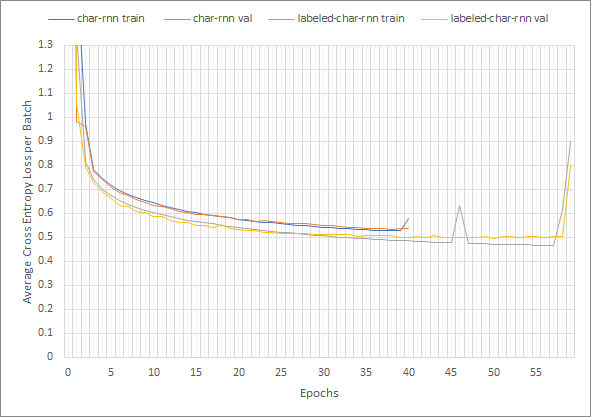
\includegraphics[trim = 2 2 2 2, clip, keepaspectratio]{images/training1.png}
	\centering
	\caption{Καμπύλες εκμάθησης για τα \en{top 100 github js projects}}
	\label{training1}
\end{figure}

\subsection{\en{Top 200 npm Projects} Πειράματα}

Το δεύτερο σετ δεδομένων αποτελείται από τις 200 πιο δημοφιλείς βιβλιοθήκες \en{javascript} του ιστοχώρου www.npmjs.com.
Οι ακολουθίες μετά την προ-επεξεργασία αριθμούν περίπου 49 εκατομμύρια χαρακτήρες με 210 διαφορετικούς χαρακτήρες. 
Σε αυτό το πείραμα χωρίζουμε το 90\% των ακολουθιών στο σετ εκπαίδευσης και το 10\% στο σετ επαλήθευσης, επειδή έχουμε λιγότερα δεδομένα και θέλουμε να αποφύγουμε μεγάλη διακύμανση στο σετ επαλήθευσης.

Οι αποφάσεις των υπερπαραμέτρων βασίζονται στις παρατηρήσεις μας από τα προηγούμενα πειράματα. Έτσι, κρατάμε ίδιο το μέγεθος παρτίδας, τον ρυθμό εκμάθησης και το μήκος ακολουθίας.
Το σετ εκπαίδευσης έχει μικρότερο μέγεθος από το προηγούμενο πείραμα και από τις πρώτες δοκιμές παρατηρούμε σημαντικό \en{overfitting}.
Προς την κατεύθυνση καλύτερης γενίκευσης των συμπερασμάτων του συστήματος, αρχικά μικραίνουμε το δίκτυο θέτοντας το μέγεθος \en{LSTM} se 700, κίνηση η οποία μειώνει σημαντικά τις εκπαιδεύσιμες παραμέτρους του συστήματος.
Έπειτα αυξάνουμε την πιθανότητα \en{dropout} σε 30\% και 40\% που αποτέλεσμα έχει την αργήτερη εκπαίδευση του αναδραστικού νευρωνικού δικτύου.
Για να αποζημιώσουμε την τελευταία μας επιλογή αυξάνουμε τις εκπαιδευτικές εποχές του μοντέλου σε 60 και 80 αντίστοιχα.
Οι εκπαιδευτικές επιλογές συνοψίζονται στον πίνακα \ref{hyper2}.

\begin{table}[]
\centering
\begin{tabularx}{\textwidth}{|X|X|X|}%TODO Check these values
\hline
                    & \en{char-rnn} & \en{labeled-char-rnn} \\
\hline
\en{\#} Παραμέτρων       & 10M             & 10M                     \\
\hline
\en{\#} Χαρακτήρων       & 210             & 210, 8                  \\
\hline
\en{\#} Εποχών       & 60             & 80                  \\
\hline
Μέγεθος \en{LSTM}  & 700            & 700                    \\
\hline
Μήκος Ακολουθίας    & 100             & 100                     \\
\hline
Ρυθμός Εκμάθησης    & 0.002           & 0.002                   \\
\hline
\% \en{Dropout}     & 30              & 40                      \\
\hline
Μέγεθος Παρτίδας    & 200             & 200                     \\
\hline
\end{tabularx}
\caption{Υπερπαράμετοι για τα \en{top 200 npm js libaries}}
\label{hyper2}
\end{table}

Η διαδικασία που ακολουθείται είναι η ίδια με του προηγούμενου πειράματος, δηλαδή εκπαιδεύουμε το σύστημα σε μία κάρτα γραφικών \en{Nvidia Gtx 960} με 4 \en{gb RAM} και επιλέγουμε το μοντέλο με τις καλύτερες επιδόσεις στη μετρική πρόβλεψης χαρακτήρων.
Η εκπαίδευση του \en{char-rnn} διαρκεί 3 ημήρες ενώ του \en{labeled-char-rnn} διαρκεί περίπου 4. Η εξέλιξη της εκπαίδευσης φαίνεται στην εικόνα \ref{training2}.

\begin{figure}[h]
	\caption{Καμπύλες εκμάθησης για τα \en{top 100 github js projects}}
	\label{training1}
	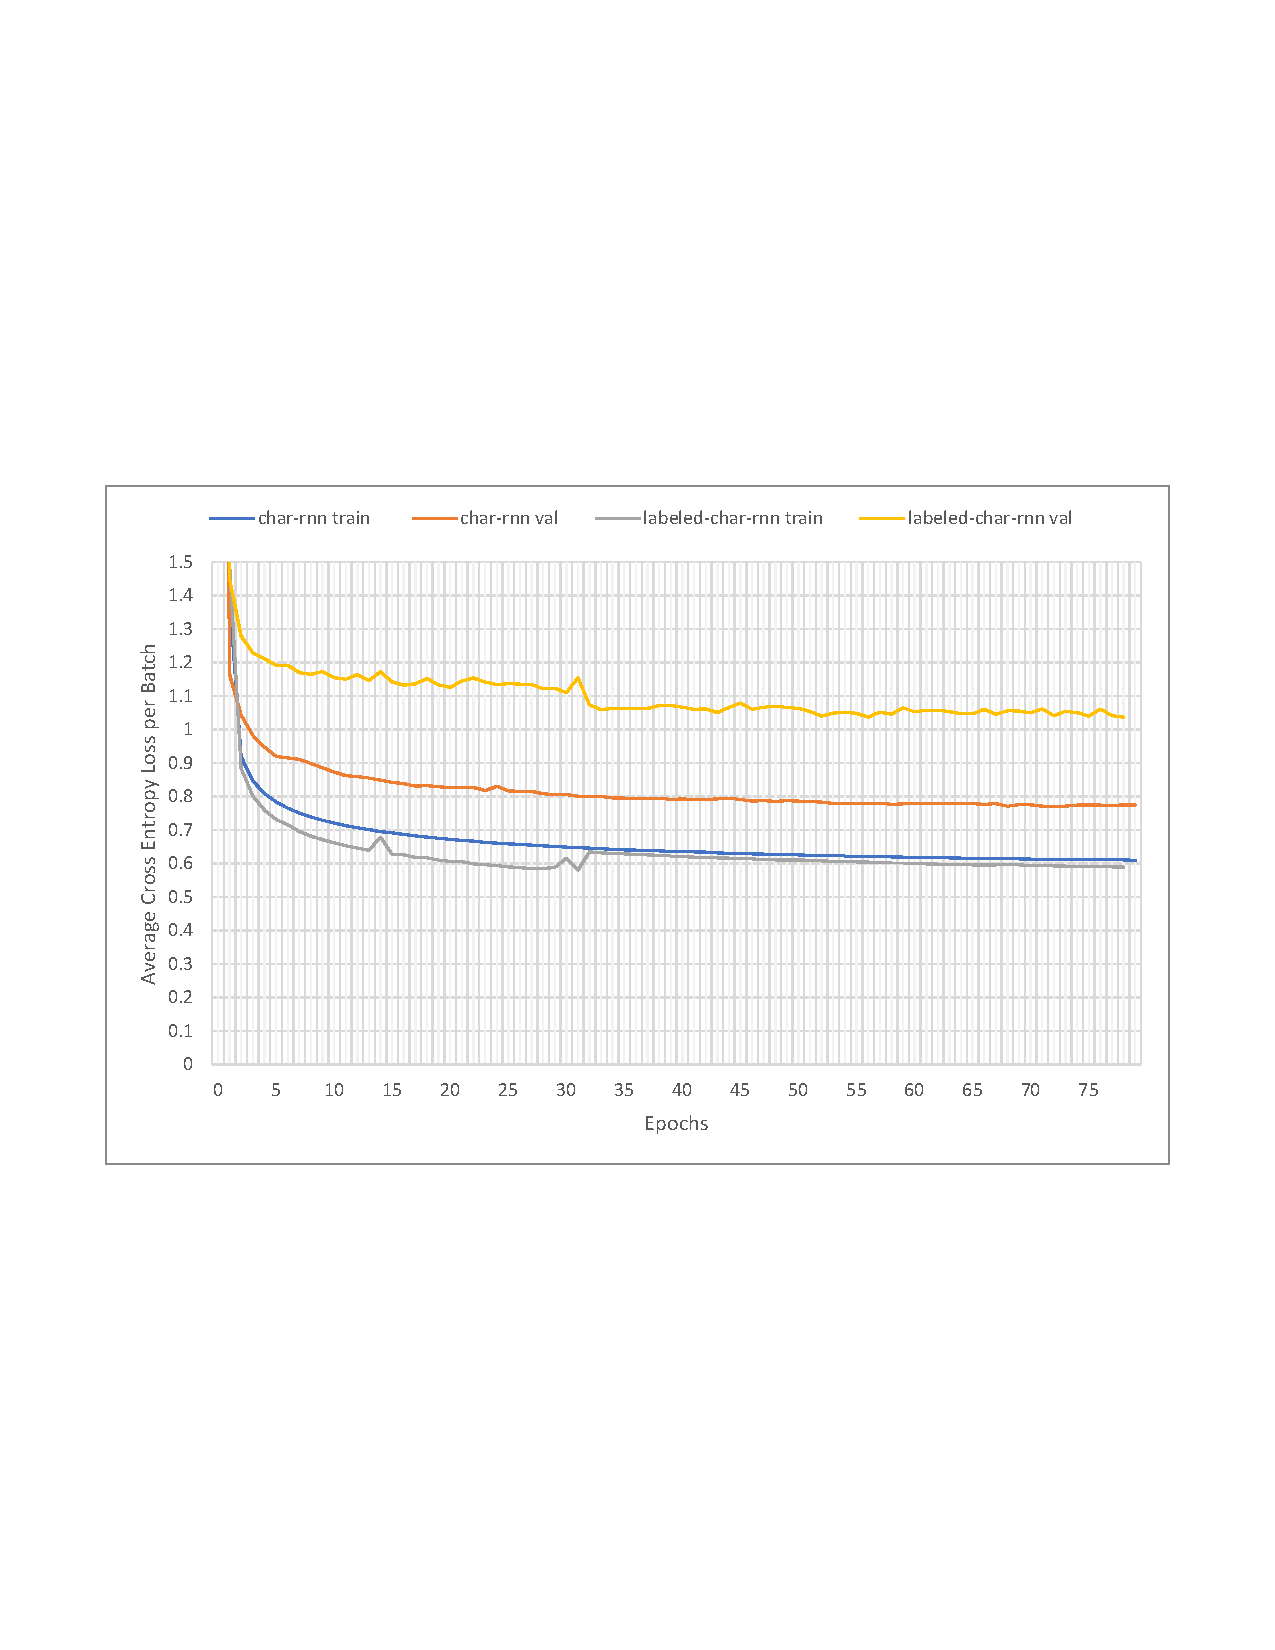
\includegraphics[width=\textwidth, trim = 25 220 25 220, clip, keepaspectratio]{images/training2.pdf}
	\centering
\end{figure}


Το επιλεγόμενο μοντέλο για το \en{char-rnn} είναι αυτό της 72ης εποχής με ποσοστό επιτυχίας πρόβλεψης 78\%. Για το μοντέλο \en{labeled-char-rnn} το επιλεγόμενο μοντέλο είναι αυτό της 78ης εποχής με ποσοστό επιτυχίας 72.3\% την πρόβλεψη χαρακτήρων και 94.7. Είναι εμφανές από το διάγραμμα οτι τα μοντέλα μας δυσκολεύονται περισσότερο να γενικεύσουν τα συμπεράσματα που εξάγουν από αυτό το σετ δεδομένων. Η ικανότητα πρόβλεψης του είδους του επόμενου χαρακτήρα παραμένει σε σχετικά υψηλά επίπεδα αλλα η προσθήκη της δεν βελτιώνει τις επιδόσεις στο σετ επιβεβαιωσης. Θα εξετάσουμε αναλυτικότερα τα αποτελέσματα αυτά στο υποκεφάλαιο των αποτελεσμάτων και στο κεφάλαιο των συμπερασμάτων.
%TODO Maybe add a side experiment subsevtion.

\section{Αποτελέσματα}

Χρησιμοποιούμε τα μοντελα που εκπαιδεύτηκαν παραπάνω για να παράξουμε 100 αρχεία κώδικα για κάθε προσέγγιση και κάθε ομάδα μοντέλων.
Επιλέγουμε ένα \en{javascript} project με το οποίο αρχικοποιούμε κάθε ομάδα μοντέλων. 
Αρχικά θα εξετάσουμε την ποιότητα του κώδικα εποπτικά και έπειτα θα χρησιμοποήσουμε το εργαλείο \en{jshint} για να κάνουμε στατική ανάλυση του κώδικα.

\subsection{\en{Top 100 Github Javascript Projects} Παραγώμενος κώδικας}

Η αρχικοποίηση του μοντέλου γίνεται με σκοπό την οδήγηση του.
Επιλέγουμε ένα project που δεν έχει εμφανιστεί στη διάρκεια της εκπαίδευσης και της επαλήθευσης.
Συγκεκριμένα επιλέγουμε το \en{hyper terminal} που είναι το πιο δημοφιλές \en{javascript project} στο \en{github} το πρώτο εξάμηνο του 2017.
Ο κώδικας 5.1 είναι ένα αρχείο από το \en{project} αυτό.

\selectlanguage{english}
\lstinputlisting[language=JavaScript, caption={\tg{Δείγμα κώδικα απο το }\en{hyper terminal}}]{code/hyper.js}
\selectlanguage{greek}

Όι κώδικες 5.2, 5.3 είναι δημιουργήματα των μοντέλων \en{char-rnn} και \en{labeled-char-rnn} αντίστοιχα. Τα αρχεία αυτά επιλέχτηκαν χάρη στο μικρό μέγεθός τους και την συντακτική ορθότητα.

\selectlanguage{english}
\lstinputlisting[language=JavaScript, caption={\tg{Δείγμα κώδικα απο το }\en{char-rnn}}]{code/charrnnGithub.js}
\selectlanguage{greek}

Ήδη εποπτικά παρατηρούμε τη δυνατότητα και των δύο μοντέλων να αναπαράγουν συντακτικές δομές, όπως οι παρενθέσεις και οι αγκύλες, αλλα και λογικές, όπως οι συναρτήσεις και οι δομές πολλαπλών επιλογών.
Φαινομενικά αυτό είναι ένα συνηθισμένο αρχείο \en{javascript}.
Με μία δεύτερη, αναλυτικότερη ματιά παρατηρούμε σημαντικά λάθη στη χρήση μη ορισμένων μεταβλητών, την ύπαρξη γραμματικών λαθών και ενέργειες χωρίς αποτέλεσμα. 
Είναι εύκολο να συμπεράνει κανείς, ίσως και χωρίς να είναι γνώστης της γλώσσας, πως τα προγράμματα αυτά δεν θα καταφέρουν να μεταφραστούν. 
Για την καλύτερη εκτίμηση των αποτελεσμάτων των νευρωνικών δικτύων, και για τη σύγκριση των δύο  θα ακολουθήσουμε μια πιο ποσοτική προσέγγιση. 
Με τη χρήση του εργαλείόυ ανάλυσης κώδικα \en{jshint} θα εξετάσουμε τον αριθμό των συντακτικών λαθών που εντοπίζονται και μέχρι πιο σημείο καταφέρνουν να αναγνωστούν πριν βρεθεί ένα ανεπανόρθωτο συντακτικό λάθος.
Σημειώνεται πως τα μοντέλα αποφασίζουν αυτόνομα το μήκος του κώδικα, με τη χρήση των ειδικών χαρακτήρων, αλλά τίθεται ένα άνω όριο 15000 χαρακτήρων στο οποίο θεωρούμε οτι το αρχείο ξεφεύγει διαχειρισμότητας λόγω μεγέθους.
Στις εικόνες \ref{static-github-char} - \ref{MCE2-githubLabeled} φαίνονται τα αποτελέσματα της παραπάνω ανάλυσης και το μήκος των παραγώμενων αρχείων.

\selectlanguage{english}
\lstinputlisting[language=JavaScript, caption={\tg{Δείγμα κώδικα απο το }\en{labeled-char-rnn}}]{code/labeledcharrnnGithub.js}
\selectlanguage{greek}

\begin{figure}[!htb]
	\caption{Στατική ανάλυση κώδικα για τα αποτελέσματα του \en{char-rnn} μοντέλου}
	\label{static-github-char}
	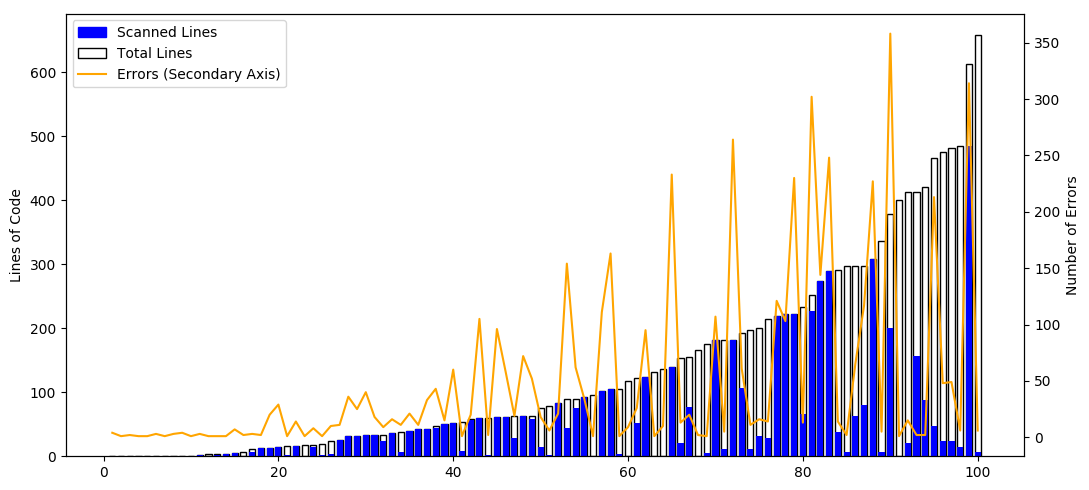
\includegraphics[width=\textwidth, keepaspectratio]{images/jshint-githubChar.png}
\end{figure}

\begin{figure}[!htb]
	\caption{Στατική ανάλυση κώδικα για τα αποτελέσματα του \en{labeled-char-rnn} μοντέλου}
	\label{static-github-labeled}
	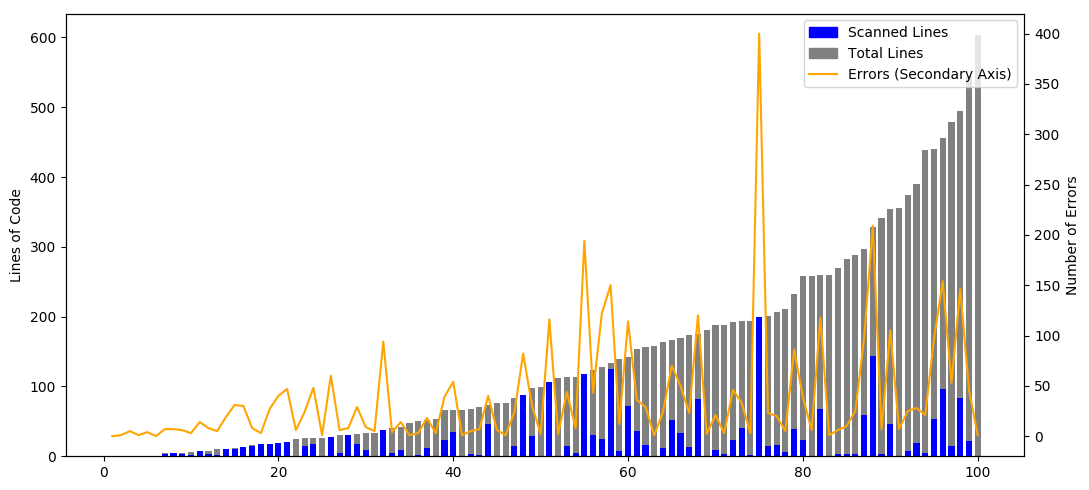
\includegraphics[width=\textwidth, keepaspectratio]{images/jshint-githubLabeled.png}
\end{figure}

\begin{figure}[!htb]
	\caption{Συνηθέστερο λάθος των αρχείων του \en{char-rnn}}
	\label{MCE1-githubchar}
	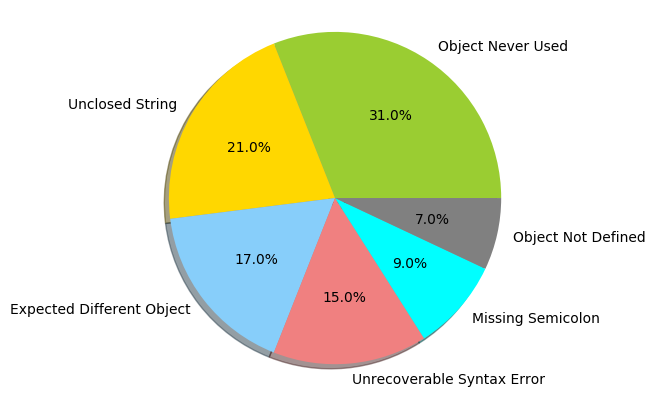
\includegraphics[width=\textwidth, keepaspectratio]{images/MCE-githubchar.png}
\end{figure}

\begin{figure}[!htb]
	\caption{Δεύτερο συνηθέστερο λάθος των αρχείων του \en{char-rnn}}
	\label{MCE2-githubchar}
	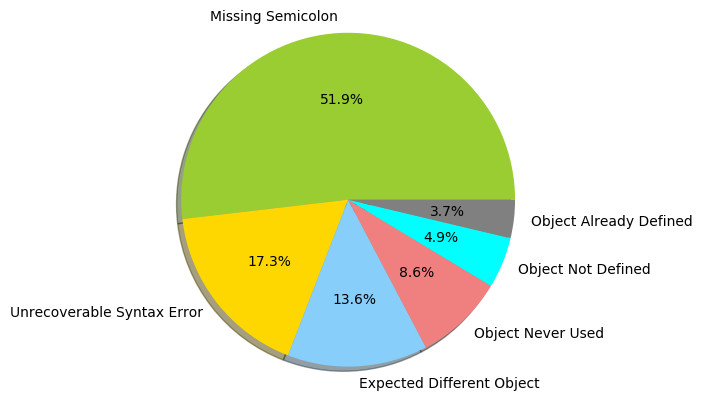
\includegraphics[width=\textwidth, keepaspectratio]{images/MCE2-githubchar.png}
\end{figure}

\begin{figure}[!htb]
	\caption{Συνηθέστερο λάθος των αρχείων του \en{labeled-char-rnn}}
	\label{MCE1-githubLabeled}
	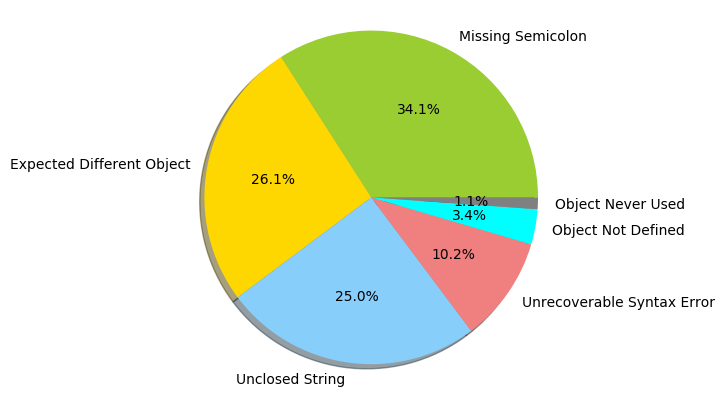
\includegraphics[width=\textwidth, keepaspectratio]{images/MCE-githubLabeled.png}
\end{figure}

\begin{figure}[!htb]
	\caption{Δεύτερο συνηθέστερο λάθος των αρχείων του \en{labeled-char-rnn}}
	\label{MCE2-githubLabeled}
	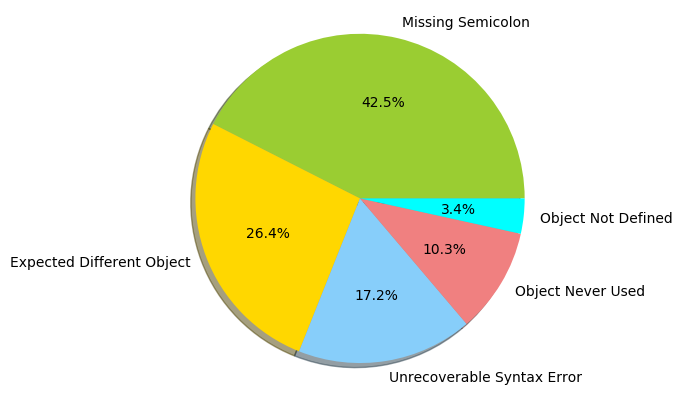
\includegraphics[width=\textwidth, keepaspectratio]{images/MCE2-githubLabeled.png}
\end{figure}

Στα σχήματα \ref{static-github-char} και \ref{static-github-labeled} μπορούμε να συγκρίνουμε τις επιδόσεις των δύο μοντέλων.
Αρχικά παρατηρούμε πως και τα δύο μοντέλα παράγουν κάποια κενά αρχεία ή αρχεία με 1 ή 2 γραμμές.
Το μέσο μήκος των αρχείών είναι αρκετά κοντινό (137.1 - 142.21 γραμμές) και το δεύτερο μοντέλο καταφέρνει να κλείσει τα αρχεία σε λιγότερο απο 15000 χαρακτήρες 9\% των φορών ενώ το πρώτο 6\%.
Αν και το δεύτερο μοντέλο έχει περισσότερη πληροφορία για τον κώδικα, παράγει αρχεία που ολοκληρώνουν την ανάλυση κώδικα με αρκετά μικρότερη συχνότητα.
Η γενική εικόνα που παίρνουμε απο την ανάλυση αυτή είναι απογοητευτική για το δεύτερο μοντέλο, που ενώ έχει στη διάθεση του περισσότερη πληροφορία αποτυγχάνει να την αποτυπώσει με τρόπο που να παράγει ποιοτικά αποτελέσματα.

Τα είδη των συνηθέστερων λαθών μαρτυρούν τις αδυναμίες της προσέγγισης μας στην παραγωγή κώδικα.
Ακόμα και αν καταφέρνουν να δημιουργήθούν μικρά κομμάτια λειτουργικού κώδικα η έλλειψη ανεξάρτητης μνήμης και η στοχαστική φύση της παραγωγής δυσκολεύουν τα μοντέλα ως προς τη διαχείριση των διαφόρων μεταβλητών, τη χρήση της σύνταξης και τη επίτευξη του τελικού σκοπού.
Αρκετά συχνά η δημιουργία αλφαριθμητικών ξεφεύγει της διαχείρισης του μοντέλου και συνεχίζεται ναγράφεται κώδικας μέσα σε κάποιο αλφαριθμητικό - που είναι ο κύριος λόγος της ύπαρξης του \en{Unclosed String}.

\subsection{\en{Top 200 npm Projects} Παραγώμενος κώδικας}

Ακολουθούμε ανάλυση όμοια με την προγούμενη υποενότητα. Το \en{project} αρχικοποίησης που χρησιμοποιείται ειναι το: 